\documentclass[11pt]{article}
\usepackage[utf8]{inputenc}
\usepackage[english, ngerman]{babel}
\usepackage{amsmath,amsthm,verbatim,amssymb,amsfonts,amscd}
\usepackage{enumerate}
\usepackage{listings}
\usepackage{courier}
\usepackage{graphicx}
\usepackage[margin=1in]{geometry}
\usepackage{epstopdf}
\lstset{
  numbers=left,
  language=C,
  basicstyle=\footnotesize\ttfamily,
  breaklines=true,
  morekeywords={function, NIL}
}
\newcommand{\abs}[1]{\left| #1 \right| }
\setlength{\parindent}{0pt} 

\author{
  Felix Schrader, 3053850 \\ 
  Jens Duffert, 2843110 \\
  Eduard Sauter, 3053470
}
\title{Datenstrukturen und Algorithmen: Haus\"ubung 4}
\begin{document}
\maketitle
\subsection*{Aufgabe 2}
\begin{figure}[h!]
  \centering
  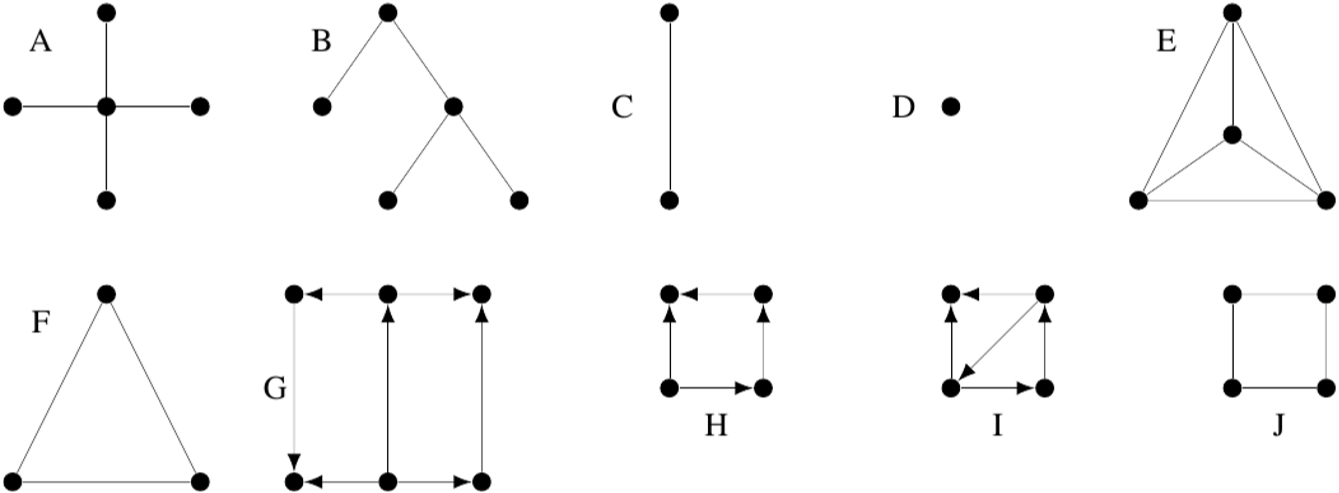
\includegraphics[width=0.8\textwidth]{a2_graphs.png}
  \caption{Graphen aus der Aufgabenstellung}
  \label{fig:a2_graphs}
\end{figure}
In Tabelle \ref{tab:table_a2} sind die Ergebnisse dieser Aufgabe noch einmal
zusammengefasst. In Abbildung \ref{fig:a2_graphs} sind die Graphen aus der Aufgabe zu
sehen.
\begin{enumerate}[a)]
  \item
    Ein freier Baum ist ein azyklischer, ungerichteter und zusammenhängender
    Graph. Alle zehn abgebildeten Graphen sind zusammenhängend. Die Graphen $G$,
    $H$ und $I$ sind gerichtet, also keine freien Bäume. Von den Verbliebenen
    haben nur $A$, $B$, $C$ und $D$ keine Zyklen, dies sind also die einzigen
    freien Bäume in diesem Beispiel.
  \item
    In einem vollständigen Graphen ist jeder Knoten mit jedem anderen verbunden.
    Dies ist bei den Graphen $C$, $D$, $E$ und $F$ der Fall.
  \item
    Ein Zyklus ist eine Folge von Knoten, die jeweils durch Kanten verbunden
    sind, wobei der erste und letzte Knoten der Folge übereinstimmen. Der Graph
    $A$, $B$, $C$ und $D$ haben wie bereits in a) erwähnt keine Zyklen (dabei
    gehen wir davon aus, dass zwei direkt miteinander verbundene Knoten wie in
    $C$ keine Zyklen sind, da sonst jeder ungerichtete Graph mit zwei Knoten
    oder mehr einen Zyklus hätte). $E$ und $F$ haben jeweils den Zyklus
    \textsf{oben - links - rechts - oben}. $G$ hat keinen Zyklus, da der Knoten
    unten in der Mitte von keinem anderen Knoten erreicht werden kann und es in
    dem Graphen, wenn man diesen Knoten entfernt, nur einen Knoten gibt, den man
    erreichen und wieder verlassen kann. Das gleiche Argument gilt bei $H$ mit
    dem Knoten unten links. In $I$ gibt es den Zyklus
    \textsf{oben rechts - unten links - unten rechts - oben rechts}. In $J$ gibt
    es den Zyklus
    \textsf{oben links - unten links - unten rechts - oben rechts - oben links}.
\end{enumerate}
\begin{table}[h!]
  \centering
  \begin{tabular}{|c|c|c|c|c|c|c|c|c|c|c|}
    \hline
    Graph & $A$ & $B$ & $C$ & $D$ & $E$ & $F$ & $G$ & $H$ & $I$ & $J$ \\
    \hline
    freier Baum & ja & ja & ja & ja & nein & nein & nein & nein & nein & nein \\
    \hline
    vollständig & nein & nein & ja & ja & ja & ja & nein & nein & nein & nein \\
    \hline
    zyklenfrei & ja & ja & ja & ja & nein & nein & ja & ja & nein & nein \\
    \hline
  \end{tabular}
  \caption{Zusammenfassung der Ergebnisse}
  \label{tab:table_a2}
\end{table}

\subsection*{Aufgabe 3}
\begin{enumerate}[a)]
  \item 
    \begin{figure}[h!]
      \centering
      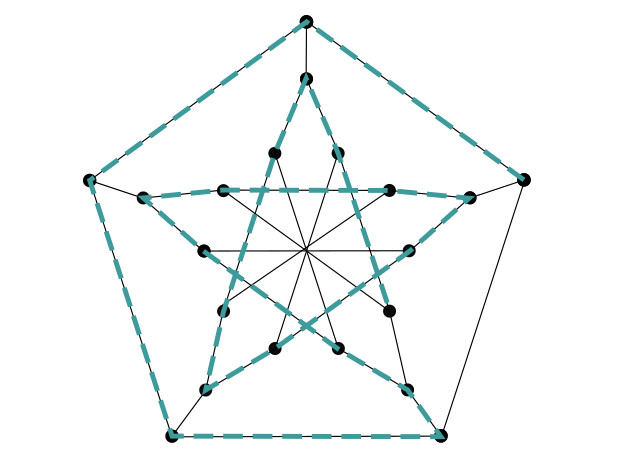
\includegraphics[width=0.8\textwidth]{hamilton_graph}
      \caption{Hamiltonischer Pfad}
      \label{fig:hamilton_graph.eps}
    \end{figure}
  \item
    Es sei $G$ ein Graph $(V, E)$ mit $\abs{V} = n>3$ Knoten.
    %
    \begin{align*}
      |E| & =\frac{n^2 - 3n}{2} + 3 = 3 - n + \sum_{i=1}^{n-1} i \\
          & = 2  + \sum_{i=1}^{n-2} i
    \end{align*}
    %
    Die Summe bezeichnet die Anzahl aller Kanten eines Vollst\"andigen 
    Graphen mit $n-1$ Knoten. Der Graph besteht also insgesamt aus einem 
    Vollst\"andigen Teilgraphen mit $n-1$ Knoten und dem geforderten Knoten
    mit 2 Kanten. In einem Vollst\"andigen Graphen, ist es trivialerweise
    m\"oglich einen Hamilton Pfad zu finden, der an zwei beliebigen 
    Punkten beginnt und endet. Da also so ein Pfad existiert, muss man
    nurnoch die Verbindungen zu dem Knoten von Grad 2 zum Pfad hinzuaddieren
    und erh\"alt auf diese Art einen Hamiltonkreis.

\end{enumerate} 

\subsection*{Aufgabe 4}
In Abbildung \ref{fig:a4_tree} ist der Baum zu sehen. In Tabelle
\ref{tab:degree_and_weight} sind Verzweigungsgrad $v$ und Gewicht $w$ der Knoten
eingetragen. Der Verzweigungsgrad ist die Anzahl der direkten Nachfolger, das
Gewicht ist die Anzahl aller Nachfolger.
\begin{figure}[h!]
  \centering
  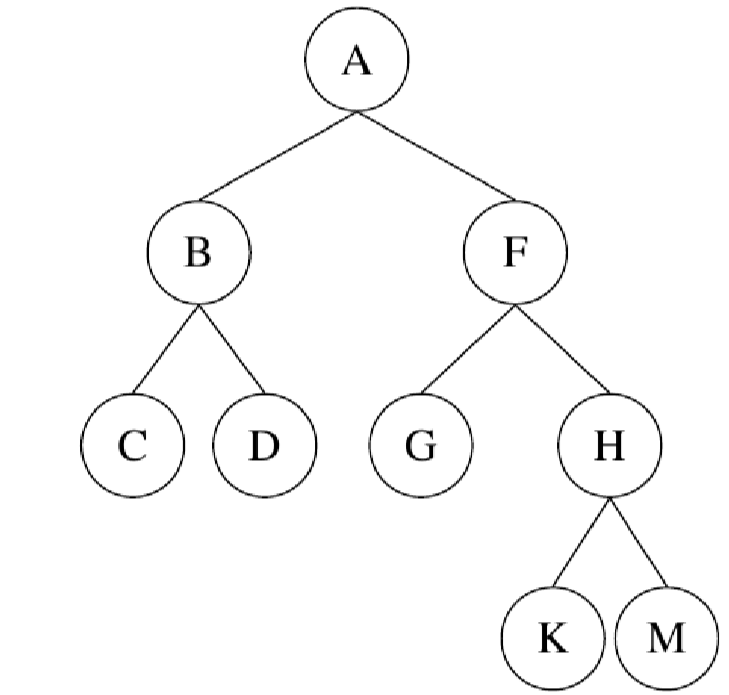
\includegraphics[width=0.4\textwidth]{a4_tree.png}
  \caption{Baum aus der Aufgabenstellung}
  \label{fig:a4_tree}
\end{figure}
\begin{table}[h!]
  \centering
  \begin{tabular}{|c|c|c|c|c|c|c|c|c|c|}
  \hline
  Knoten & $A$ & $B$ & $C$ & $D$ & $F$ & $G$ & $H$ & $K$ & $M$ \\
  \hline
  $v$ & 2 & 2 & 0 & 0 & 2 & 0 & 2 & 0 & 0 \\
  \hline
  $w$ & 8 & 2 & 0 & 0 & 4 & 0 & 2 & 0 & 0 \\
  \hline
  \end{tabular}
  \caption{Verzweigungsgrad und Gewicht der Knoten}
  \label{tab:degree_and_weight}
\end{table}

\end{document}
